\subsection{FAST}


Segundo \cite{FAST}, � um m�todo de reconhecimento baseado em detec��o de
arestas originalmente desenvolvido por Edward Rosten e Tom Drummond. A maior
promessa do m�todo � a efici�ncia computacional. O m�todo considera um c�rculo
de dezesseis pixels ao redor da aresta considerada p.
O detector original \cite{FusingPoints},\cite{VideoAnotation} classifica p como
uma aresta se existirem n pixels cont�guos em um c�rculo que s�o mais brilhantes
do que o pixel candidato de intensidade Ip mais um threshold t ou mais escuros do que Ip-t

 \begin{figure}[h!]
\centering
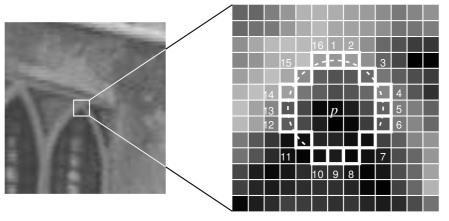
\includegraphics[scale=0.8]{images/fast01}
\caption{FAST}
\label{fig:fast01}
\end{figure}


Na imagem~\ref{fig:fast01} foi escolhido n=12. Um teste r�pido �
\begin{enumerate}
	\item Selecionar o ponto � testar primeiro as extremidades. No caso da imagem,
	escolhido o ponto p
	\item Comparar os pontos 1 e 9, e verificar se o ponto p tem intensidade
	com diferen�a de m�dulo t, ou seja os pontos 1 e 9 s�o mais claros ou mais escuros do que o ponto p pelo fator de t
	\item Avaliar se o ponto p continue sendo um candidato considerando os pontos 5
	e 13
	\item Analisar se p � uma aresta, sendo pelo menos 3 desses pontos devem ser
	mais brilhantes ou mais escuros do que p ent�o o teste pode ser feito nos demais pontos.
\end{enumerate}

